\documentclass[a4paper, 11pt]{scrreprt}
\usepackage[swedish]{babel}
\usepackage[utf8]{inputenc}
\usepackage[T1]{fontenc}
\usepackage{lmodern}
\usepackage{euler}

\usepackage{amsfonts}
\usepackage{amsmath}

\usepackage{fancyhdr}
\usepackage{graphicx}

\usepackage{scrhack}
\usepackage[table]{xcolor}
\usepackage{listings}
\usepackage{float}
\usepackage{tabularx}
\usepackage{lastpage}
\usepackage{smartref}
\usepackage[nice]{units}
\usepackage{sidecap}
\usepackage{blindtext}
\usepackage{pdflscape}
\usepackage{parskip}
\usepackage{subcaption}
\usepackage{natbib}
\usepackage{tikz}
\usetikzlibrary{shapes,arrows}

\usepackage{hyperref}
%centrera alltid bilder
\makeatletter
\g@addto@macro\@floatboxreset{\centering}
\makeatother

\hypersetup{
colorlinks=true
}

% Fin header
\pagestyle{fancy}
%\fancyhf{}
\renewcommand{\chaptermark}[1]{\markboth{\thechapter.\space#1}{}}
\lhead{\sffamily Design av Robothand}
%\rhead{\sffamily Sida \thepage\ av \pageref{LastPage}}
\rhead{\sffamily \leftmark}


\newcommand\measurepage{\dimexpr\pagegoal-\pagetotal-\baselineskip\relax}
\definecolor{light-gray}{gray}{0.95}

\let\oldtabularx\tabularx
\let\endoldtabularx\endtabularx
\renewenvironment{tabularx}{\rowcolors{2}{white}{light-gray}\oldtabularx}{\endoldtabularx}


\newcommand{\comment}[1]{\textcolor{blue}{[#1]}}


\title{Design av Robothand - Slutrapport}



\begin{document}


\section{Sammanfattning}

Följande är en rapport som beskriver  "Design av robothand" som går ut på att konstruera en mekanisk hand som styrs trådlöst med en styrhandske, där användarens rörelser efterliknas av robothanden. Robothanden känner även av hur mycket de greppade föremålet påverkas med hjälp av trycksensorer vilket ger en återkoppling av handens gripkraft.

Med utgångspunkt i liknande arbeten framtas en grundläggande mekanisk princip  som används för att konstruera de separata fingrarna. För att manipulera fingrarna används sex stycken hobbyservon som kontrollerar fingrarna via senor och stag. För att få en uppfattning (om möjligt, hitta bättre ord än “uppfattning”) om handens utseende, funktionalitet och rörelse används CAD-ritningar och rörelsesimuleringar innan tillverkning. 

Kommunikationen mellan styrhandsken och robothanden upprättas med hjälp av mikrokontrollers, så kallade Arduinokort. Signalerna från styrhandsken reglerar robothandens rörelse och fås från flexgivare* som sitter på styrhandsken.
Mikrokontrollerna styr även de hobbyservon som i sin tur får robothanden att röra sig.
\chapter{Inledning}

\section{Inledning}

Robothänder kan användas som ett mycket effektivt hjälpmedel, inte bara för personer i behov av en protes, utan även i industriella tillämpningar. Monotona, fysiskt tunga, och direkt farliga arbeten kan utföras av en robothand istället för en människa.  Det pågår idag mycket forskning och utveckling av robothänder och detta har resulterat i mycket avancerade prototyper. En av de mest avancerade just nu är Shadow Dexterious Hand (TM) som med sina 20 aktuerade frihetsgrader och totalt 129 sensorer kan utföra det mesta som man kan begära av en mänsklig hand (ref längst ner). Stora hinder i utvecklingen generellt har varit de höga kostnaderna, den komplexa fingerfärdigheten samt styrning. Kostnaden för en hand som kan efterlikna den mänskliga handens rörelser överstiger ofta 10 000 dollar (ref längst ner). Kostnaden stiger i regel med ökat antal kontrollerbara frihetsgrader och ökad komplexitet. 
 

Möjligheten att fjärrstyra robothänder innebär att olika arbeten eller uppgifter kan utföras av en expert utan att experten finns på plats. Denna möjlighet kan vara direkt livräddande vid till exempel uppgiften att desarmera en bomb. Ett problem med att fjärrstyra en robothand är att operatören inte själv kan känna föremålet som hanteras vilket lätt kan leda till att ett för hårt eller löst grepp appliceras. Detta kan i sin tur resultera i att föremålet skadas eller i extremfallet, att en bomb detoneras. Vidare är det problematiskt att få styrningen att kännas intuitiv genom till exempel knapptryckningar. 

%Föregående stycke är inte klart /Chris

\subsection{Syfte} %Eller snarare "Contributions".
I denna rapport redogörs för utvecklingen av en robothand som fjärrstyrs med hjälp av en styrhandske, där alltså robothanden skall röra sig som operatörens hand. Genom att designa robothanden för att likna mänskliga handen i sina rörelser blir styrningen intuitiv. För att undvika skador på objekt som robothanden hanterar ska ett bibliotek av objekt kunna implementeras i robothandens mikrokontroller som möjliggör objektidentifiering. Varje objekt har ett fördefinierat högsta tryck som robothanden får utsätta den för. Om operatören försöker greppa hårdare än det fördefinierade trycket ska robothanden reglera detta för att undvika skada. 
Objektidentifieringen är baserad på igenkänning av objektets storlek genom att utifrån servovinklarnas positioner beräkna avståndet mellan de tryckbelastade punkterna på robotfingrarna vid greppning.

Systemets principiella funktion kanske ska in här? %tycker bengt


För att uppnå detta krävs... (redogör för mål) %enligt Bengts råd. Jonas tycker mål passar bättre i planeringsrapport, samtidigt som han tycker att vi borde placera greppbilderna under rubriken mål istället för där vi har dem i mittrapporten... oklart.)

\subsection{Avgränsningar}
Budgeten för projektet är 5000 kr.

\subsection{Rapportens Upplägg}
Rapporten är upplagd som följer..
I kapitel hmm till hmm ges en beskrivning av systemets design och funktion. Först diskuteras den mekatroniska designen av robothanden för att belysa dess rörelseomfång. I nästkommande kapitel behandlas styrhandsken med mikrokontroller och elektriska kretsar i detalj. Slutligen i kapitel hmm redogörs vilka algoritmer som utvecklats för att uppnå styrning och reglering.

I kapitel hmm finns resultat... efter dessa följer disskusion om bla bla och bla slutligen en slutsats där våra mål verifieras.





\subsection{Projektdefiniton} %Ta bort denna rubrik tror jag

\subsection{Avgränsningar}



\subsection{Vad inledningen ska innehålla enligt anvisningar}
Inledningen sätter in rapporten i ett sammanhang och visar dess
relevans och nyhetsvärde. Den fungerar som en introduktion till
hela rapporten och ska ge läsaren nödvändig information som
behövs för att ta del av dess innehåll.
Inledningen innehåller normalt en syftesformulering som ofta
ställs i relation till en bakgrund eller kort historik. I många fall
är syftesformuleringen nära relaterad till den
problemformulering som är viktig för att såväl läsare som
skribent ska kunna utnyttja rapporten väl. Det bör också stå
något om undersökningens eller experimentets omfattning och
anledningar till särskilda avgränsningar. Vidare bör också
metod finnas med, men endast i syfte att ange vilken typ av
undersökning som gjorts. Metoden utvecklas i andra avsnitt av
rapporten.
Man brukar ange bakgrund, syfte och metod som inledningens
obligatoriska funktioner. Ibland signaleras även centrala resultat
redan i inledningen.
Inledningen är den första sidan som sidnumreras.



http://www.shadowrobot.com/products/dexterous-hand/

http://www.nytimes.com/2013/03/30/science/making-robots-mimic-the-human-hand.html?_r=0



\chapter{Metod och material}
I detta avsnitt kommer den konstruerade robothanden och dess delfunktioner att presenteras. Först presenteras en systemöverblick på funktionell nivå och därefter presenteras ingående komponenter.
\chapter{Metod och material}
I detta avsnitt kommer den konstruerade robothanden och dess delfunktioner att presenteras. Först presenteras en systemöverblick på funktionell nivå och därefter presenteras ingående komponenter.

\section{Robothand}

I detta avsnitt presenteras en överblick över de komponenter som utgör den mekaniska handen. Handens mekaniska delar utgörs till största delen av standardiserade komponenter från en Meccano™ byggsats. 
\begin{figure}[H]
\includegraphics[width=0.90\textwidth]{img/hand}
\caption{Handen och dess delkomponenter.}
\end{figure}
Handen består av två fingrar och en tumme som beskrivs utförligare i sina respektive avsnitt nedan. På fingrar och tumme sitter det även plastskal som har som uppgift att skapa bättre greppytor. På samtliga fingertoppar finns trycksensorer som kan mäta relativa normalkrafter. En Arduino Due mikrokontroller styr de sex stycken servomotorer som aktuerar fingrarna och sköter även kommunikationen via bluetooth med styrhandsken för att ta emot styrsignaler samt skicka uppmätta trycksensorvärden.   
 Handen har aktuatorer, mikrokontroller, bluetooth och strömförsörjning integrerat i en enda enhet.\\
Fingrarnas rörelseomfång och relativa position tillåter ett stort antal olika grepp, med olika krav på styrka, omfång, finkänslighet och fingerfärdighet. 
\begin{figure}[H]
\includegraphics[width=0.90\textwidth]{img/provagrepp}
\caption{Verifiering av relativ fingerpositionering utefter greppförmåga.}
\label{fig:cad}
\end{figure}
Handens design verifieras i CAD-miljö innan konstruktion för att på ett effektivt sätt säkerhetsställa att ett flertal olika objekt kan gripas. Figur~\ref{fig:cad} illustrerar hur handen griper olika objekt av varierande storlek och form.

%I figuren ovan syns de utprovade greppen, som i sin tur kan identifieras i Cutkoskys grepphierarki. %%Se \ref{cutkosky} 
%Då handen konstruerats för att kunna hantera både stora och små objekt som kräver  både greppstyrka och finmotorik är den mycket flexibel vilket gör att den säkert kan greppa och hantera objekt av olika storlekar och tyngd.



\subsection{Fingrar och tumme}
Handens två identiska fingrar är designade för  att efterlikna ett människolikt rörelsemönster vilket underlättar för användaren då rörelsemönstret hos robothanden imiterar det mänskliga.


\begin{figure}[H]
\includegraphics[height=0.3\textheight]{img/fingerbild}
\label{oversiktsbild}
\caption{Översiktsbild fingerdesign.}
\label{fig:finger}
\end{figure}

Fingrarna har tre leder varav Led 1 och Led 2 (se figur~\ref{fig:finger}) är separat styrbara. Led 3 är via ett stag tvångsstyrd av Led 2 för att imitera hur ett mänskligt finger beter sig när handen sluts. Jämfört med det mänskliga fingret saknas förmågan att vid Led 1 vrida fingret i sidled. Beskrivning av hur fingrar och tumme aktueras finns i avsnitt~\ref{Kraftovf} Kraftöverföring\\En fördel med två separat styrbara leder är att fingrarnas rörelseomfång och funktionella förmåga utökas.
\begin{figure}[H]
\includegraphics[width=0.50\textwidth]{img/1vs2frihets}
\caption{En vs. två styrbara leder.}
\label{fig:tvaleder}
\end{figure}

I figur~\ref{fig:tvaleder} demonstreras hur två styrbara leder spänner upp ett fält av möjliga positioner för fingertoppen att befinna sig i för varje läge handen står i, vilket minskar behovet av att flytta hela handen vid små justeringar av grepp, medans ett finger med endast en styrbar led tvingas följa en unik bana.\\
\\
\begin{figure}[H]
\includegraphics[height=0.15\textheight]{img/tummecad}
\caption{Tummen}
\label{fig:tumme}
\end{figure} 
Tummen (figur~\ref{fig:tumme}) skiljer sig från de två fingrarna och har endast två leder varav båda är separat styrda. I likhet med fingrarna sitter den fast positionerad i handen för att utgöra ett mothåll för finger 1 och 2 vid normalt användande och kan även göra ett pincettgrepp med finger 1 vid precisionsgrepp. Detta är tillräckligt för möjliggöra ett flertal olika grepp, men jämfört med den mänskliga tummen som kan möta samtliga fingertoppar är detta ett stelt utförande.





\subsubsection{Fingertoppar och sensorer}
För att insamla information om hur hårt handen påverkar objekt som hanteras sitter det trycksensorer längst ut på varje fingertopp.
\begin{figure}[H]
\includegraphics[height=0.3\textheight]{img/trycksensor}

\caption{Beskrivning}
\label{fig:trycksensor}
\end{figure}
I figur~\ref{fig:trycksensor} ovan syns trycksensorns position på fingertoppen. Trycksensorerna är av modell Interlink 0.5 FSR 100N, och kan mäta kontakttryck på den cirkulära ytan i spannet 0.11-110 MPa. Mätningen sker genom att ytan komprimeras, vilket resulterar i en minskad resistans hos trycksensorn, som registreras av handens mikrokontroller. Sensorerna kan dock endast uppskatta ett tryck i normalriktningen, ingen information om vart på sensorytan, eller hur stort område som belastas kan återges, vilket resulterar i att endast relativa krafter kan mätas, då ett flertal olika tryckbelastningar med varierande utbredning över sensorytan kan resultera i samma resistansminskning.
\begin{figure}[H]
\includegraphics[height=0.25\textheight]{img/sensor}
\caption{Monterad fingertopp med trycksensor under gummi}
\label{fig:monteradtopp}
\end{figure}
Över sensorerna sitter ett 3 mm tjockt lager av syntetiskt gummi (se figur~\ref{fig:monteradtopp}) för att skydda samt ge större friktion vid hantering av objekt.\\
\begin{figure}[H]
\includegraphics[height=0.30\textheight]{img/pincett}
\caption{Tumme och finger 1 håller en nyckel i pincettgrepp.}
\label{fig:pincett}
\end{figure}
Fingertopparna är utformade för att kunna skapa ett pincettgrepp vid hantering av små känsliga objekt där kontatktrycket mäts, se figur~\ref{fig:pincett}.
Nedre delen av fingertoppen fungerar som stöd vid övrig grepp men där mäts inte kontakttrycket. Fingertopparna skapas i CAD och skrivs ut i en 3d-printer.
\section{Aktuering}
I detta avsnitt presenteras servomotorer och kraftöverföring.\\
Totalt har handen åtta leder varav sex är separat styrbara. Varje styrbar led aktueras av en servomotor. Kraftöverföringen mellan servomotor och finger sker med stag och genomlöpande senor. 
\subsection{Servon}
Aktuatorer för samtliga leder är sex stycken Blue Bird BMS-660DMG+HS (se figur~\ref{fig:servo}) och är så kallade hobbyservon.
\begin{figure}[H]
\includegraphics[height=0.2\textheight]{img/servo}
\caption{Blue Bird BMS-660DMG+HS servo.}
\label{fig:servo}
\end{figure}
 Dessa servomotorer används för att de uppfyller kraven på vridmoment med god marginal (se APPENDIX A.HIYTF för dimensionerande beräkningar). Vid en matningsspänning på 6 Volt har servot ett maximalt vridmoment på 1.42 Nm och en högsta rotationshastighet på 6.16 rad/s utan belastning. Servona har ett totalt rörelseomfång på 120 grader vilket är standard för hobbyservos. Servona regleras via PWM-signaler och har en intern positionsreglering, detta gör att servomotorerna alltid arbetar för att nå det önskade läget och återgår till detta läge efter en eventuell störning.

\subsection{Kraftöverföring}
\label{Kraftovf}
Led 1 i samtliga fingrar och tumme aktueras via stag, vilket gör att de kan föras fram och tillbaka av respektive servo.

\begin{figure}[H]
\includegraphics[width=0.9\textwidth]{img/stagsenor}
\caption{Översiktsbild kraftöverföring mellan servomotorer och leder.}
\label{stagsenor}
\end{figure}
För att aktuera Led 2 används en sena som löper igenom fingret se ~\ref{fig:finsen} . Senan utgörs av en fiskelina dimensionerad för en dragkraft på 330 N. Största dragkraften i senan uppstår då servomotorn arbetar vid maximalt vridmoment och uppgår till 118 N med 12 mm servohorn. För att återföra fingret till sitt räta läge används en vridfjäder som sitter runt led 2. 

\begin{figure}[H]
\includegraphics[height=0.30\textheight]{img/fingersena}
\caption{Senans väg genom fingret.}
\label{fig:finsen}
\end{figure}


\section{Styrhandske}

\begin{figure}[H]
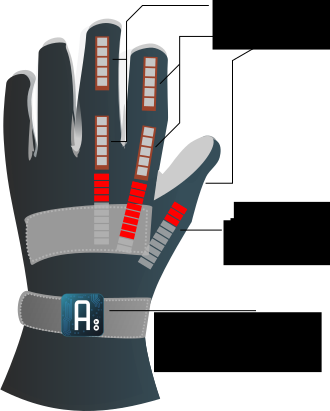
\includegraphics[height=0.5\textheight]{img/kontrollhandske}
\caption{Konceptskiss över styrhandsken}
\end{figure}

För att intuitivt reglera robothanden används en vanlig handske som användaren bär på sin hand. På tumme, långfinger och pekfinger finns det två flexsensorer vardera. Flexsensorerna ändrar resistans beroende på hur böjda de är, vilket leder till  

 vilket används för att översätta de tre fingrarnas läge till önskvärda vinklar för robothandens fingrar. När resistansen ändras, 

 ändrad resistans $\to$ ändrad spänning $\to$ spänningen normaliseras mot fingrarnas referens $\to$ önskvärd vinkel skickas till robothanden


% För att reglera robothanden används en reglerhandske som användaren har på sin hand, detta ger en intuitivt reglering (se figur). På tumme, pekfinger och långfinger på handsken sitter två flexsensorer var som följer användarens hand och ändrar resistans beroende på hur mycket de böjs. Denna resistansförändring använder man som insignal till mikrokontrollen som sitter på reglerhandsken, som i sin tur skickar styrsignaler till mikrokontrollen på robothanden. Se \ref{sec:mikro}. 

% Handsken är gjord av textil och flexsensorerna är insydda i små påsar som underlättar montering av sensorerna på handsken. (Se figur)
% (Bild på handsken)  
\section{Trådlös kommunikation}
\section{Signalbehandling}
\section{Mikrokontroller}
\label{sec:mikro}
info om våra microcontroller. Bluetooth moduelerna och hur det programmerats samt hur det fungerar.
\section{Elektriska kretsar}
\begin{figure}[H]
\includegraphics[height=0.5\textheight]{img/schemahandske}
\caption{Kopplingsschema för styr/regler-handsken.}
\end{figure}
\begin{figure}[H]
\includegraphics[height=0.5\textheight]{img/schemahand}
\caption{Kopplingsschema för robothanden.}
\end{figure}


Figur \ref{} visar hur styrhandsken är kopplad. Komponenterna är lödda på ett experimentkort.

\section{Algoritmer}
Här presenteras de styralgortimter som bestämmer hur handen beter sig när den följer användarens input samt identifierar och greppar objekt. 
\subsection{Objektidentifiering}
\begin{figure}[H]
EN BILD SOM FÖRKLARAR DETTA, SAMT VILKA OBJEKT VI VALT ATT identifierar och hur vi gör det...
\caption{Beskrivning}
\end{figure}
Antaganden: Servona står i önskat läge, det vill säga tidsfördröjningen som uppstår då servona skall vrida sig från godtycklig position till den önskade antags vara så liten vid normalt användande att den kan försummas. Då ingen mätning av servonas verkliga position görs, är den enda informationen om fingrarnas lägen det önskade servoläget. 

FIXA FLÖDESSSCHEMA OCH ETT ARDUINO PROGRAM Känner av tryck (över visst gränsvärde) på tumme och motstående finger->, lagrar användarens input läge då detta inträffar ( för att när användaren går utanför detta igen (öppnar sin hand) så skall handen återgår till att följa användaren) -> beräknar avståndet mellan sensorerna-> checkar av avståndet mot en lista av fördefinerade objekt som innehåller , storlek och önskat trycksensorvärde med en +/-tolerans för att inte handen ska stå och flippa som en tok för att uppnå EXAKT rätt värde-> TADAA!!-> när användaren öppnar sina fingrar utanför "kontaktläget" följer handen efter igen...
Mer teksti


\chapter{Resultat}
\chapter{Resultat}
För att verifiera robothandens funktion kontrolleras objektidentifieringen, samt om robothanden kan begränsa trycket mellan robothandens fingrar och objektet då identifiering gjorts. Detta test ställer krav på den mekaniska konstruktionen, trådlösa överföringen, sensorerna i styrhandsken och robothanden samt att den matematiska modellen fungerar. Med andra ord behöver hela systemet fungera och samverka väl för att uppnå ett bra resultat.

Efter utförda funktionstester har följande resultat uppnåtts. Robothanden kan:
\begin{itemize}
\item Gripa och lyfta ett mjölkpaket med en vikt av ett kg. 
\item Gripa och lyfta en mutter av storlek M10 mellan tumme och pekfinger. 
\item Lyfta en last motsvarande ett kg på mitten av två fingrar.
\item Lyfta upp en snusdosa.
\item Sluta sig till knuten näve från öppen hand på under en sekund.
\end{itemize}

\subsection{Objektidentifiering}
För att kunna identifiera objekt behöver den matematiska modellen som beskriver hur robothandens fingrar är positionerade överensstämma med den faktiska konstruktionen av robothanden. 
\begin{figure}[H]
\includegraphics{img/obj_id_matlab2}
\caption{Avståndet mellan det faktiska och beräknade värdet.}
\label{avstand}
\end{figure}

Figur~\ref{avstand} visar hur den matematiska modellen avviker från ett perfekt mätresultat för 18 olika mätningar. Det genomsnittliga felet är 20 procent och inom handens typiska arbetsområde, som är \unit{40-200}{mm}, är felet endast i genomsnitt 11 procent med ett största fel på \unit{15}{mm}. Utgående från detta som största felmarginal kan robothanden med säkerhet särskilja objekt som har \unit{15}{mm} differens på det klassificerande måttet.

Med denna väljas två olika testobjekt ut för att kontrollera om robothanden kan särskilja dem. det kan den och alla blir glada och dricker sprit och knullar. THE END

\chapter{Diskussion}
\section{Diskussion}
En underliggande tanke med projektet var att robothanden kunde vara en grund för vidareutveckling i kommande kandidatarbeten. Då systemet i sin helhet innehåller så många ingenjörsmässiga områden, men tiden är begränsad, har fokus legat främst på att få till en fungerande helhet snarare än att specialutveckla eller optimera en viss del som exempelvis den mekansika konstruktionen eller objektidentifieringen. Det har antagits att Meccanot kommer hålla för de uppgifter robothanden ska utföra varför projektet avgränsade behovet av hållfasthetsberäkningar. Objektidentifieringen är begränsad till två dimensioner, alltså bara tummen och pekfingrets lägen är med i beräkningarna. 

Ett av de stora problemen med styrning av robothanden och dess precision vid identifiering av objekt är stabiliteten i kontruktionen. Tidigt i projektet togs beslutet att handen skulle byggas i meccano för att snabbt åstadkomma en prototyp och börja utveckla och testa styrningen. Att bygga i meccano resulterade i glapp mellan olika delar och töjningar av materialet som inte räknades med i den matematiska modellen. Detta gör att en korrekt bedömning av avståndet mellan fingertopparna för att identifiera objekt får låg precision varför antalet objekt som kan implementeras i programmet kraftigt begränsas (och målet att identifiera tre olika objekt inte uppnådes om detta ska va ett mål). Problem med skruvar som lossnar och delar som blir sneda gjorde dessutom att styrningsresultat kunde skilja sig från en gång till en annan. Detta innebär att en kalibrering av servomotorernas läge för greppning av ett bestämt objekt behövdes oftare än tänkt. Konstruktionen fungerar i övrigt bra. 

%Trots att det lagts mer tid på projektet än tänkt så har inte alla mål uppnåtts. Mycket tid i projektet har gått åt till att försöka få tag på personer på skolan som kan hjälpa till med att få tag på material som multimeter, resistanser, spänningsregulatorer m.m eller för att fråga om råd inom vissa områden där kandidatgruppens kompitens har varit bristande. Detta problem skulle kunna undvikas om material fanns tillgängligt i exempelvis ett lab där det även finns en ansvarig som kan vara till hjälp då det är problem med materialet. 
%Andra orsaker till förseningar har varit att olika saker går sönder. Exempelvis blev signalbehandlingsarbetet uppskjutet då många trycksensorer och flexsensorer gick sönder. Detta berodde till stor del på vår okunskap om deras ömtålighet. Problemet hade kunnat undvikas dels genom att vara försiktigare men också genom att i förväg köpa in reserver.

%Om ett liknande kandidatarbete ska göras i framtiden rekommenderas att en tydligare projektram tillhandahålls från början. Vi försökte under lång tid i början på projektet hålla många dörrar öppna och undvek att noga precisera målet med projektet.  Att sätta upp projektets mål och syfte visade sig vara mycket svårt då bedömningen av svårigheten i att uppnå vissa egenskaper eller tiden det tar att utföra uppgifter, grundas på kandidatgruppens kunskap. Målen har därför behövts alterneras allt eftersom. Man kan visserligen lära sig av detta problem men det tog mycket fokus från det tekniska arbetet. Ett mer välutstakat syfte med projektet skulle ge högre motivationsnivå.

 
 


 



\end{document}
